\section{Auswertung}
\label{sec:Auswertung}
\subsection{Bragg-Bedingung}
Zunächst wurde wie in Bereich \ref{sec:bragg} bereits beschrieben, die Bragg-Bedingung überprüft.
Dafür wird der Kristall und das Rohr entsprechend positioniert wodurch die Messwerte in Tabelle \ref{tab:bragg} aufgenommen wurde.
Wie zu erkennen ist liegt das Maximum der Impulse pro Sekunde bei einem Winkel von $\theta = 28.2 \si{\degree} $ wobei $N = 218.0 \frac{\text{Imp}}{\si{\second}}$ ist.
Die Werte sind zudem in der Grafik \ref{fig:bragg} aufgetragen worden.
Der Plot dafür, sowie alle folgenden Plots wurden mit dem python Plugin \cite{matplotlib} erstellt.
\begin{table}
  \centering
  \caption{Die Messwerte die zur Überprüfung der Bragg-Bedingung aufgenommen wurden.}
  \begin{tabular}[t]{cc}
  \toprule
  $\theta \,/\, \si{\degree}$ & $N \,/\, \frac{\text{Imp}}{\si{\second}}$ \\ 
  \midrule
    26.0	&   56.0\\
    26.1	&   58.0\\
    26.2	&   54.0\\
    26.3	&   62.0\\
    26.4	&   58.0\\
    26.5	&   68.0\\
    26.6	&   72.0\\
    26.7	&   83.0\\
    26.8	&   89.0\\
    26.9	&   95.0\\
    27.0	&   105.0\\
    27.1	&   119.0\\
    27.2	&   125.0\\
    27.3	&   141.0\\
    27.4	&   154.0\\
    27.5	&   157.0\\
    27.6	&   166.0\\
    27.7	&   180.0\\
    27.8	&   188.0\\
    27.9	&   211.0\\
    28.0	&   212.0\\
  \bottomrule
\end{tabular}
\begin{tabular}[t]{cc}
  \toprule
  $\theta \,/\, \si{\degree}$ & $N \,/\, \frac{\text{Imp}}{\si{\second}}$ \\ 
  \midrule
    28.1	&   215.0 \\
    28.2    &	218.0\\
    28.3    &	215.0\\
    28.4    &	208.0\\
    28.5    &	189.0\\
    28.6    &	189.0\\
    28.7    &	176.0\\
    28.8    &	164.0\\
    28.9    &	149.0\\
    29.0    &	138.0\\
    29.1    &	125.0\\
    29.2    &	111.0\\
    29.3    &	107.0\\
    29.4    &	95.0\\
    29.5    &	77.0\\
    29.6    &	73.0\\
    29.7    &	58.0\\
    29.8    &	56.0\\
    29.9    &	53.0\\
    30.0    &	53.0\\
  \bottomrule
  \end{tabular}
  \label{tab:bragg}
\end{table}

\begin{figure}
    \centering
    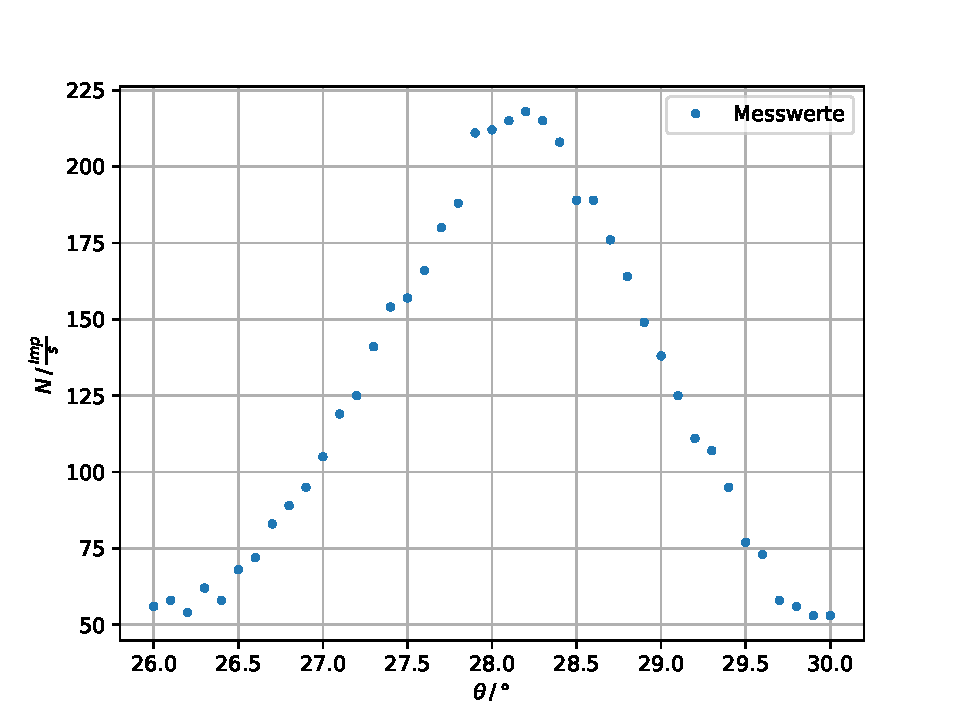
\includegraphics[width=\textwidth]{content/data/absorption1.pdf}
    \caption{Die gemessenen Intensitäten in Abhängigkeit vom Winkel $\theta$.}
    \label{fig:bragg}
\end{figure}

\FloatBarrier

\subsection{Emissionsspektrum einer Kupferröntgenröhre}


In den Tabellen \ref{tab:emission1} und \ref{tab:emmision2} sind die Messwerte zu finden, welche bei der Messung des Spektrums der Kupferröntgenröhre aufgenommen wurden.
Der Ablauf der Messung ist im Abschnitt \ref{sec:emission} zu sehen.
Die Werte wurden zudem in Grafik \ref{fig:emis} aufgetragen.
Die gemessenen Impulse pro Sekunde wurden dabei in Abhängigkeit vom Winkel $\theta$ aufgetragen.
Der Bremsberg, sowie die $K_\alpha$ und $K_\beta$-Linie wurden markiert.
Zudem wurde die Halbwertsbreite ($FWHM$) angenähert.
Dafür wurden bei jedem Peak die Werte ausgewählt, die am nächsten an der Hälfte des Maximums des entsprechenden Ordinaten-Wertes liegen.
Darauf wurden die zwei Werte dessen $\theta$ Wert kleiner als der des Maximums ist, durch eine Gerade verbunden.
Das selbe geschah mit den Werten dessen $\theta$ Wert größer dem des Maximums ist.
Danach wurden die beiden Geraden durch eine Gerade verbunden, die parallel zur Abzissenachse steht.
Diese befindet sich genau auf der Höhe des halben Ordinaten-Werts des Maximums.
Die Länge dieser Gerade entspricht der Halbwertsbreite.
Der Wert der beiden Halbwertsbreite lässt sich so auf
\begin{align*}
    FWHM(K_\beta) &=  0.4947 \si{\degree} \\
    FWHM(K_\alpha) &=  0.4938 \si{\degree} \\
\end{align*}
bestimmen.
Aus diesen lässt sich nun eine Energiedifferenz $\Delta E_\text{FWHM}$ berechnen mit der anschließend das Auflösungsvermögen ermittelt werden kann.
Dafür werden mithilfe der Gleichung \eqref{eq:bragg} und \eqref{eq:eng}, die beiden Halbwertsbreite zunächst in Wellenlängendifferenzen und dann in die entsprechenden Energiedifferenz umgerechnet.
Nun kann durch die Division der Maximalen Energie der Linie $E_\text{K}$ und der Energiedifferenz $\Delta E_\text{FWHM}$ das zuvor genannt Auflösungsvermögen bestimmt werden.
Dies liegt bei den gegebenen Messwerten bei 
\begin{align*}
    A_\beta &= 48.5054 \\
    A_\alpha &=  43.0748. \\
\end{align*}
Zusätzlich wurden die Abschrimkonstanten $\sigma_1$ bis $\sigma_3$ bestimmt.
Dafür wurde die Gleichung
\begin{equation*}
  E_\text{K,abs} = R_\infty (z-\sigma_1)^2
  \label{eq:sigma1}
\end{equation*}
nach $\sigma_1$ umgestellt.
Zusätzlich musste der Wert für $E_\text{K,abs}$ recherchiert werden, da dieser mit gegebenen Versuchsaufbau nicht zu ermitteln ist.
Der Literaturwert aus Quelle \cite{xray} beträgt $E_\text{K,abs} = 8.9789 \si{\kilo\eV}$. 
So ergibt sich ergibt sich für die Abschrimkonstante der Wert $\sigma_1 = 3.2925$.
Aus diesem Wert kann mit Hilfe von
\begin{equation*}
  E_{\text{K},\alpha} = R_\infty (z-\sigma_1)^2 - R_\infty \frac{1}{2^2}(z-\sigma_2)^2,
\end{equation*}
der Wert der Abschrimkonstante $\sigma_2 = 12.3331$ bestimmt werden.
Dabei ist $E_{\text{K},\alpha} = \SI{1.2887e-18}{\joule}$ die maximale Energie der Strahlung der $K_\alpha$-Linie.
Zuletzt wird $\sigma_3$, aus den beiden bereits berechneten Abschrimkonstanten errechnet.
Dafür wird die Gleichung 
\begin{equation*}
  E_{\text{K},\beta} = R_\infty (z-\sigma_1)^2 - R_\infty \frac{1}{3}(z-\sigma_3)^2
\end{equation*}
genutzt.
Hier ist $E_{\text{K},\beta} = \SI{1.4282e-18}{\joule}$ die maximale Energie der Strahlung der $K_\beta$-Linie.
Die Werte der drei Abschrimkonstanten sind demnach 
\begin{align*}
\sigma_1 =& 3.2925 \\
\sigma_2 =& 12.3331 \\
\sigma_3 =& 22.0126. \\
\end{align*}

\begin{figure}
  \centering
  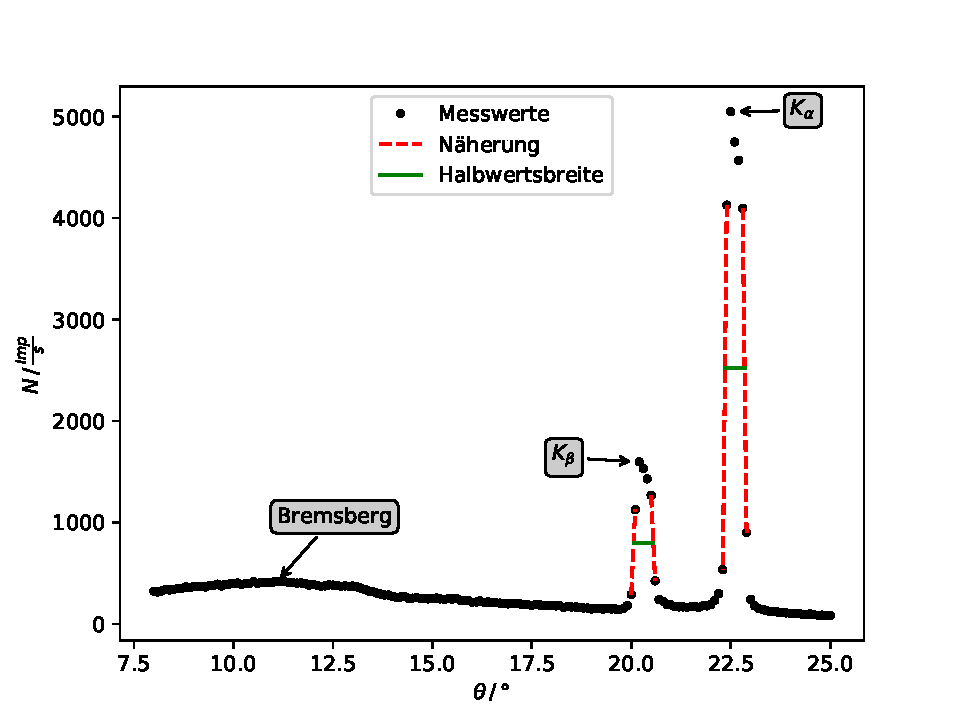
\includegraphics[width=\textwidth]{content/data/spektrum.pdf}
  \caption{Das Spektrum der Cu-Röntgenröhre, mit Halbwertsbreiten sowie $K_\alpha$ und $K_\beta$-Linien.}
  \label{fig:emis}
\end{figure}

\begin{table}
\centering
  \caption{Die aufgenommen Intensitäten der Röntgenröhre nach Reflexion an einem LiF-Kristall [Teil 1].}
  \begin{tabular}[t]{cc}
  \toprule
  $\alpha \,/\, \si{\degree} $ & $\frac{N}{\text{Imp}/\si{\second}}$\\
  \midrule
  8.0 & 323.0 \\
  8.1 & 316.0\\
  8.2 & 326.0\\
  8.3 & 340.0\\
  8.4 & 335.0\\
  8.5 & 343.0\\
  8.6 & 350.0\\
  8.7 & 350.0\\
  8.8 & 366.0\\
  8.9 & 357.0\\
  9.0 & 371.0\\
  9.1 & 371.0\\
  9.2 & 372.0\\
  9.3 & 364.0\\
  9.4 & 381.0\\
  9.5 & 379.0\\
  9.6 & 393.0\\
  9.7 & 375.0\\
  9.8 & 391.0\\
  9.9 & 395.0\\
  10.0 & 402.0\\
  10.1 & 405.0\\
  10.2 & 390.0\\
  10.3 & 398.0\\
  10.4 & 400.0\\
  10.5 & 418.0\\
  10.6 & 401.0\\
  10.7 & 410.0\\
  10.8 & 408.0\\
  \bottomrule
  \end{tabular}
  \begin{tabular}[t]{cc}
  \toprule
  $\alpha \,/\, \si{\degree} $ & $\frac{N}{\text{Imp}/\si{\second}}$ \\
  \midrule
  10.9 & 409.0\\
  11.0 & 414.0\\
  11.1 & 420.0\\
  11.2 & 417.0\\
  11.3 & 417.0\\
  11.4 & 409.0\\
  11.5 & 406.0\\
  11.6 & 404.0\\
  11.7 & 405.0\\
  11.8 & 400.0\\
  11.9 & 383.0\\
  12.0 & 389.0\\
  12.1 & 382.0\\
  12.2 & 372.0\\
  12.3 & 376.0\\
  12.4 & 385.0\\
  12.5 & 384.0\\
  12.6 & 382.0\\
  12.7 & 373.0\\
  12.8 & 376.0\\
  12.9 & 373.0\\
  13.0 & 375.0\\
  13.1 & 366.0\\
  13.2 & 354.0\\
  13.3 & 341.0\\
  13.4 & 326.0\\
  13.5 & 318.0\\
  13.6 & 305.0\\
  13.7 & 296.0  \\
  \bottomrule
  \end{tabular}
  \begin{tabular}[t]{cc}
  \toprule
  $\alpha \,/\, \si{\degree} $ & $\frac{N}{\text{Imp}/\si{\second}}$ \\
  \midrule
  13.8 & 286.0  \\
  13.9 & 285.0  \\
  14.0 & 274.0  \\
  14.1 & 264.0  \\
  14.2 & 266.0  \\
  14.3 & 270.0  \\
  14.4 & 255.0  \\
  14.5 & 255.0  \\
  14.6 & 260.0  \\
  14.7 & 251.0  \\
  14.8 & 250.0  \\
  14.9 & 248.0  \\
  15.0 & 253.0  \\
  15.1 & 257.0  \\
  15.2 & 248.0  \\
  15.3 & 242.0  \\
  15.4 & 249.0  \\
  15.5 & 246.0  \\
  15.6 & 252.0  \\
  15.7 & 236.0  \\
  15.8 & 234.0  \\
  15.9 & 231.0  \\
  16.0 & 215.0  \\
  16.1 & 217.0  \\
  16.2 & 227.0  \\
  16.3 & 214.0  \\
  16.4 & 217.0  \\
  16.5 & 210.0  \\
  \bottomrule
  \end{tabular}
  \label{tab:emission1}
\end{table}

\begin{table}
  \centering
  \caption{Die aufgenommen Intensitäten der Röntgenröhre nach Reflexion an einem LiF-Kristall [Teil 2].}
  \begin{tabular}[t]{cc}
  \toprule
  $\alpha \,/\, \si{\degree} $ & $\frac{N}{\text{Imp}/\si{\second}}$ \\
  \midrule
  16.6 & 211.0  \\
  16.7 & 206.0  \\
  16.8 & 205.0  \\
  16.9 & 198.0  \\
  17.0 & 203.0  \\
  17.1 & 199.0  \\
  17.2 & 198.0  \\
  17.3 & 191.0  \\
  17.4 & 192.0  \\
  17.5 & 184.0  \\
  17.6 & 191.0  \\
  17.7 & 188.0  \\
  17.8 & 181.0  \\
  17.9 & 185.0  \\
  18.0 & 184.0  \\
  18.1 & 179.0  \\
  18.2 & 180.0  \\
  18.3 & 166.0  \\
  18.4 & 173.0  \\
  18.5 & 167.0  \\
  18.6 & 169.0  \\
  18.7 & 160.0  \\
  18.8 & 159.0  \\
  18.9 & 157.0  \\
  19.0 & 149.0  \\
  19.1 & 153.0  \\
  19.2 & 150.0  \\
  19.3 & 147.0  \\
  19.4 & 150.0\\
  \bottomrule
  \end{tabular}
  \begin{tabular}[t]{cc}
  \toprule
  $\alpha \,/\, \si{\degree} $ & $\frac{N}{\text{Imp}/\si{\second}}$ \\
  \midrule
  19.5 & 148.0\\
  19.6 & 149.0\\
  19.7 & 143.0\\
  19.8 & 153.0\\
  19.9 & 182.0\\
  20.0 & 291.0\\
  20.1 & 1127.0\\
  20.2 & 1599.0\\
  20.3 & 1533.0\\
  20.4 & 1430.0\\
  20.5 & 1267.0\\
  20.6 & 425.0\\
  20.7 & 241.0\\
  20.8 & 225.0\\
  20.9 & 192.0\\
  21.0 & 188.0\\
  21.1 & 172.0\\
  21.2 & 168.0\\
  21.3 & 169.0\\
  21.4 & 166.0\\
  21.5 & 170.0\\
  21.6 & 174.0\\
  21.7 & 164.0\\
  21.8 & 180.0\\
  21.9 & 179.0\\
  22.0 & 191.0\\
  22.1 & 232.0\\
  22.2 & 300.0\\
  22.3 & 536.0\\
  \bottomrule
  \end{tabular}
  \begin{tabular}[t]{cc}
  \toprule
  $\alpha \,/\, \si{\degree} $ & $\frac{N}{\text{Imp}/\si{\second}}$ \\
  \midrule
  22.4 & 4128.0\\
  22.5 & 5050.0\\
  22.6 & 4750.0\\
  22.7 & 4571.0\\
  22.8 & 4097.0\\
  22.9 & 901.0\\
  23.0 & 244.0\\
  23.1 & 179.0\\
  23.2 & 151.0\\
  23.3 & 145.0\\
  23.4 & 130.0\\
  23.5 & 121.0\\
  23.6 & 126.0\\
  23.7 & 117.0\\
  23.8 & 112.0\\
  23.9 & 110.0\\
  24.0 & 105.0\\
  24.1 & 106.0\\
  24.2 & 107.0\\
  24.3 & 95.0\\
  24.4 & 94.0\\
  24.5 & 100.0\\
  24.6 & 91.0\\
  24.7 & 85.0\\
  24.8 & 88.0\\
  24.9 & 83.0\\
  25.0 & 85.0\\
  \bottomrule
  \end{tabular}
  \label{tab:emmision2}
\end{table}
\FloatBarrier

\subsection{Absorptionspektren}
In diesem Abschnitt werden die aufgenommen Werte aus Teil \ref{sec:abso} ausgewertet.
Die aufgenommenen Werte sind in den Tabllen \ref{tab:znba}, \ref{tab:brrb} und \ref{tab:srzr} zu finden.
Die Werte wurden zusätzlich im Plot \ref{fig:versch} dargstellt.
Die Werte die als $K$-Kanten Messwert genutzt wurden, wurden dabei mit einem 'X' markiert.
Zunächst wurden die Energieen der Absorptionskanten $E_\text{K}$ ermittelt.
Dafür wurde aus den aufgenommenen Werten das Maximum der Intensität sowie das Minimum der selben ermittelt.
Dies geschah für jeden Absorber.
Durch diese Werte konnte die Intensität in der Mitte der Kante $I_\text{K}$ berechnet werden.
Nun wurde aus den Werten, der Messwert herarausgesucht, welcher am nächsten an dem berrechneten Wert $I_\text{K}$ liegt.
Mit Hilfe des so ermittelten $\theta$-Wertes kann die Absorptionsenergie $E_\text{K,abso}$ berechnet werden.
So ergeben sich die folgenden Absorptionsenergieen
\begin{align*}
E_\text{Zink} & = \SI{1.5381e-18}{\J} \\
E_\text{Gallium} & = \SI{1.6491e-18 }{\J}\\
E_\text{Brom} & = \SI{2.1596e-18 }{\J} \\
E_\text{Rubidium} & = \SI{2.4115e-18}{\J} \\
E_\text{Strontium} & = \SI{2.5615e-18}{\J}  \\
E_\text{Zirkonium} & = \SI{2.8399e-18}{\J}.  \\
\end{align*}
Aus diesen lassen sich widerum die jeweiligen Abschrimkonstanten ermitteln.
Dies geschieht mit Glechung \eqref{eq:enkkante}.
Die Abschrimkonstanten der Metalle sind folgende
\begin{align*}
  \sigma_\text{Zink} & = 3.6345   \\
  \sigma_\text{Gallium} & = 3.7135 \\
  \sigma_\text{Brom} & = 3.8365 \\
  \sigma_\text{Rubidium} & = 4.1091 \\
  \sigma_\text{Strontium} & = 4.1202\\ 
  \sigma_\text{Zirkonium} & = 4.3729.\\
\end{align*}
Zur Bestimmmung der Rydbergenergie wurden nun die gewurzelte Energie der $K$-Kante in Abhängigkeit von der Ordnungszahl geplottet.
Dieser Plott ist in Abbildung \ref{fig:ausgleich} zu sehen.
Um nun $R_\infty$ zu bestimmen wurden die Werte durch eine Regressionsgerade angenähert.
Die Regressionsgerade wurde nach dem Muster $f(x) = ax+b$ erstellt.
Zum erstellen der Gerade wurde das Python Plugin scipy \cite{scipy} genutzt.
Die beiden Konstanten $a$ und $b$ konnten so ermittelt werden und haben einen Wert von 
\begin{align*}
  a =& \SI{1.413(11)e-09}{\sqrt{\J}}\\
  b=& \SI{-3.2(4)e-09}{\sqrt{\J}}.\\
\end{align*}
Die Rydbergenergie lässt sich nun aus dem Quadrat von $a$ bestimmen und beträgt $R_\infty = \SI{12.47(20)}{\eV}$.


\begin{figure}
  \centering
  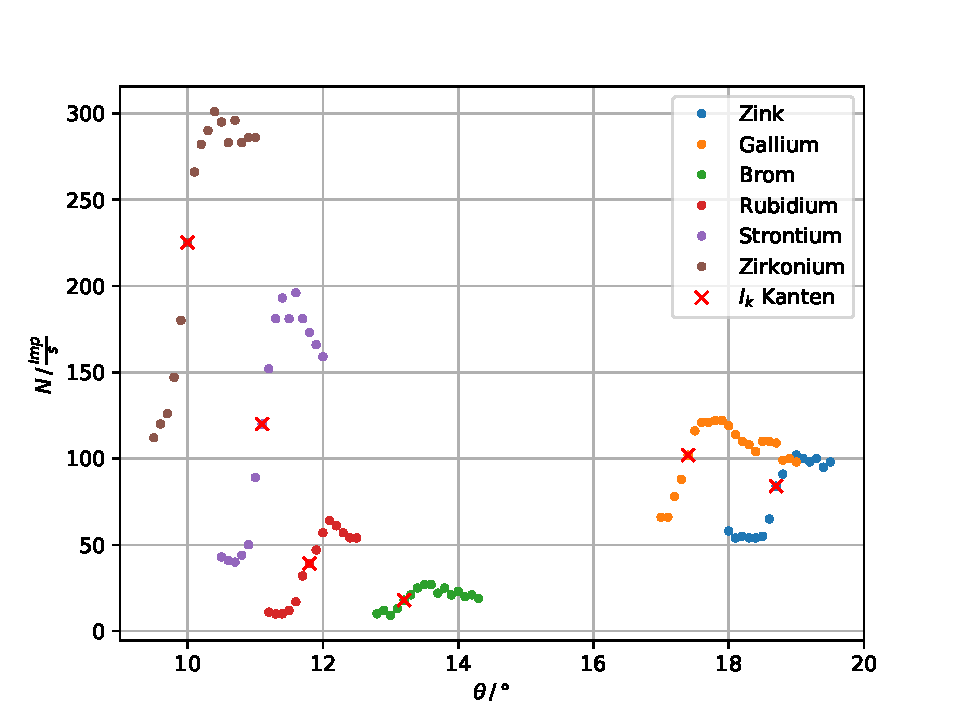
\includegraphics[width=\textwidth]{content/data/verschmetalle.pdf}
  \caption{Die verschiedenen Absorptionsspektren der Metalle, sowie die markierten Werte für die $K$-Kanten.}
  \label{fig:versch}
\end{figure}

\begin{figure}
  \centering
  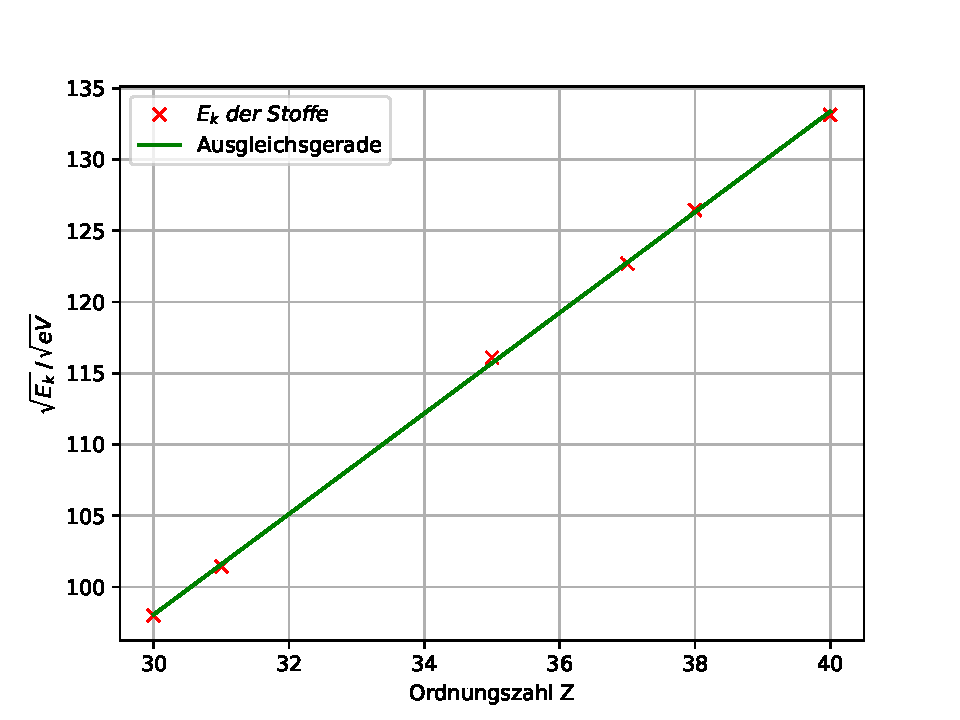
\includegraphics[width=\textwidth]{content/data/ausgleichsgerade.pdf}
  \caption{Die Ausgleichsgerade durch die gewurzelten Energiewerte der $E_\text{K}$-Linien in abhängigkeit von der Ordnungszahl.}
  \label{fig:ausgleich}
\end{figure}
%Zink, Gallium
\begin{table}
\centering
    \caption{Absorptionsspektrum von Zink (links) und Gallium (rechts).}
    \begin{tabular}{S S}
    \toprule
    $\theta \, / \, \si{\degree}$ & $N_\text{Zn} \, / \, \si{\frac{\text{Imp}}{\second}}$ \\
    \midrule
    18.0 & 58.0 \\
    18.1 & 54.0 \\
    18.2 & 55.0 \\
    18.3 & 54.0 \\
    18.4 & 54.0 \\
    18.5 & 55.0 \\
    18.6 & 65.0 \\
    18.7 & 84.0 \\
    18.8 & 91.0 \\
    18.9 & 100.0 \\
    19.0 & 102.0 \\
    19.1 & 100.0 \\
    19.2 & 98.0 \\
    19.3 & 100.0 \\
    19.4 & 95.0 \\
    19.5 & 98.0 \\
         &      \\
         &      \\
         &      \\
         &      \\
         &      \\
    \bottomrule
    \end{tabular}
    \begin{tabular}{S S}
    \toprule
    $\theta \, / \, \si{\degree}$ & $N_\text{Ga} \, / \, \si{\frac{\text{Imp}}{\second}}$ \\
    \midrule
    17.0 & 66.0 \\
    17.1 & 66.0 \\
    17.2 & 78.0 \\
    17.3 & 88.0 \\
    17.4 & 102.0 \\
    17.5 & 116.0 \\
    17.6 & 121.0 \\
    17.7 & 121.0 \\
    17.8 & 122.0 \\
    17.9 & 122.0 \\
    18.0 & 119.0 \\
    18.1 & 114.0 \\
    18.2 & 110.0 \\
    18.3 & 108.0 \\
    18.4 & 104.0 \\
    18.5 & 110.0 \\
    18.6 & 110.0 \\
    18.7 & 109.0 \\
    18.8 & 99.0 \\
    18.9 & 100.0 \\
    19.0 & 98.0 \\
    \bottomrule
    \end{tabular}
    \label{tab:znba}
\end{table}

%Brom, Rubidium
\begin{table}
\centering
    \caption{Absorptionsspektrum von Brom (links) und Rubidium (rechts).}
    \begin{tabular}{S S}
    \toprule
    $\theta \, / \, \si{\degree}$ & $N_\text{Br} \, / \, \si{\frac{\text{Imp}}{\second}}$ \\
    \midrule
    12.8 & 10.0 \\
    12.9 & 12.0 \\
    13.0 & 9.0 \\
    13.1 & 13.0 \\
    13.2 & 18.0 \\
    13.3 & 21.0 \\
    13.4 & 25.0 \\
    13.5 & 27.0 \\
    13.6 & 27.0 \\
    13.7 & 22.0 \\
    13.8 & 25.0 \\
    13.9 & 21.0 \\
    14.0 & 23.0 \\
    14.1 & 20.0 \\
    14.2 & 21.0 \\
    14.3 & 19.0 \\
    \bottomrule
    \end{tabular}
    \begin{tabular}{S S}
    \toprule
    $\theta \, / \, \si{\degree}$ & $N_\text{Rb} \, / \, \si{\frac{\text{Imp}}{\second}}$ \\
    \midrule
    11.2 & 11.0 \\
    11.3 & 10.0 \\
    11.4 & 10.0 \\
    11.5 & 12.0 \\
    11.6 & 17.0 \\
    11.7 & 32.0 \\
    11.8 & 39.0 \\
    11.9 & 47.0 \\
    12.0 & 57.0 \\
    12.1 & 64.0 \\
    12.2 & 61.0 \\
    12.3 & 57.0 \\
    12.4 & 54.0 \\
    12.5 & 54.0 \\
         &      \\
         &      \\
    \bottomrule
    \end{tabular}
    \label{tab:brrb}
\end{table}

%Strontium, Zirkonium
\begin{table}
\centering
    \caption{Absorptionsspektrum von Strontium (links) und Zirkonium (rechts).}
    \begin{tabular}{S S}
    \toprule
    $\theta \, / \, \si{\degree}$ & $N_\text{Sr} \, / \, \si{\frac{\text{Imp}}{\second}}$ \\
    \midrule
    10.5 & 43.0 \\
    10.6 & 41.0 \\
    10.7 & 40.0 \\
    10.8 & 44.0 \\
    10.9 & 50.0 \\
    11.0 & 89.0 \\
    11.1 & 120.0 \\
    11.2 & 152.0 \\
    11.3 & 181.0 \\
    11.4 & 193.0 \\
    11.5 & 181.0 \\
    11.6 & 196.0 \\
    11.7 & 181.0 \\
    11.8 & 173.0 \\
    11.9 & 166.0 \\
    12.0 & 159.0 \\
    \bottomrule
    \end{tabular}
    \begin{tabular}{S S}
    \toprule
    $\theta \, / \, \si{\degree}$ & $N_\text{Zr} \, / \, \si{\frac{\text{Imp}}{\second}}$ \\
    \midrule
    9.5 & 112.0 \\
    9.6 & 120.0 \\
    9.7 & 126.0 \\
    9.8 & 147.0 \\
    9.9 & 180.0 \\
    10.1 & 266.0 \\
    10.2 & 282.0 \\
    10.3 & 290.0 \\
    10.4 & 301.0 \\
    10.5 & 295.0 \\
    10.6 & 283.0 \\
    10.7 & 296.0 \\
    10.8 & 283.0 \\
    10.9 & 286.0 \\
    11.0 & 286.0 \\
         &       \\
    \bottomrule
    \end{tabular}
    \label{tab:srzr}
\end{table}